% =============================================================================
% Generalizacion a otros drones (version simple, ejemplos-primero).
% Sustituye la antigua seccion zero-shot. Usa solo dos figuras:
%   zeroshot_comparativa.png  y  zeroshot_recall_barras.png
% (copiadas a memoria_yolo/figuras/resultados/ desde los artefactos zeroshot).
% =============================================================================
\section{Generalización a otros drones no vistos en el entrenamiento}
\label{sec:zeroshot}

Hasta aquí el detector se ha entrenado y evaluado únicamente con el DJI Mini~3. Surge entonces una pregunta natural: ¿lo que ha aprendido sirve para otros drones, o solo sabe reconocer al Mini~3? Para responderla se hace una prueba directa: se toma el detector ya entrenado, \emph{sin reentrenarlo ni ajustar nada}, y se le pasan espectrogramas de tres drones que nunca participaron en el entrenamiento ---un DJI~F450, un Mavic~Pro y un Hunter---, capturados al aire libre. Si el detector es capaz de localizar las ráfagas de estos drones desconocidos, será señal de que ha aprendido a reconocer la \emph{forma} de una transmisión FHSS en general, y no la firma concreta del Mini~3.

La distinción tiene una consecuencia práctica importante. Un lector de paquetes convencional necesitaría conocer y decodificar el protocolo de enlace de cada modelo de dron; en cambio, un detector que reconoce la forma de la señal funciona con cualquier dron que transmita de manera parecida, aunque emplee otro protocolo o una frecuencia distinta. Los tres drones de la prueba transmiten además en frecuencias centrales separadas entre \SI{30}{\mega\hertz} y \SI{50}{\mega\hertz} de la del entrenamiento, de modo que la prueba mide también si el detector depende de la posición absoluta en frecuencia.

\subsection{Cómo detecta las ráfagas de cada dron}
\label{sec:zeroshot_ejemplos}

La \cref{fig:zeroshot_comparativa} muestra la respuesta del detector ante un espectrograma representativo de cada plataforma. En el F450 y el Mavic~Pro el detector dibuja cajas rojas ---predicción \emph{drone}--- justo sobre las ráfagas FHSS, exactamente igual que hacía con el Mini~3, a pesar de no haberlos visto nunca durante el entrenamiento. En el Hunter, en cambio, no dibuja ninguna caja de dron.

\begin{figure}[htbp]
    \centering
    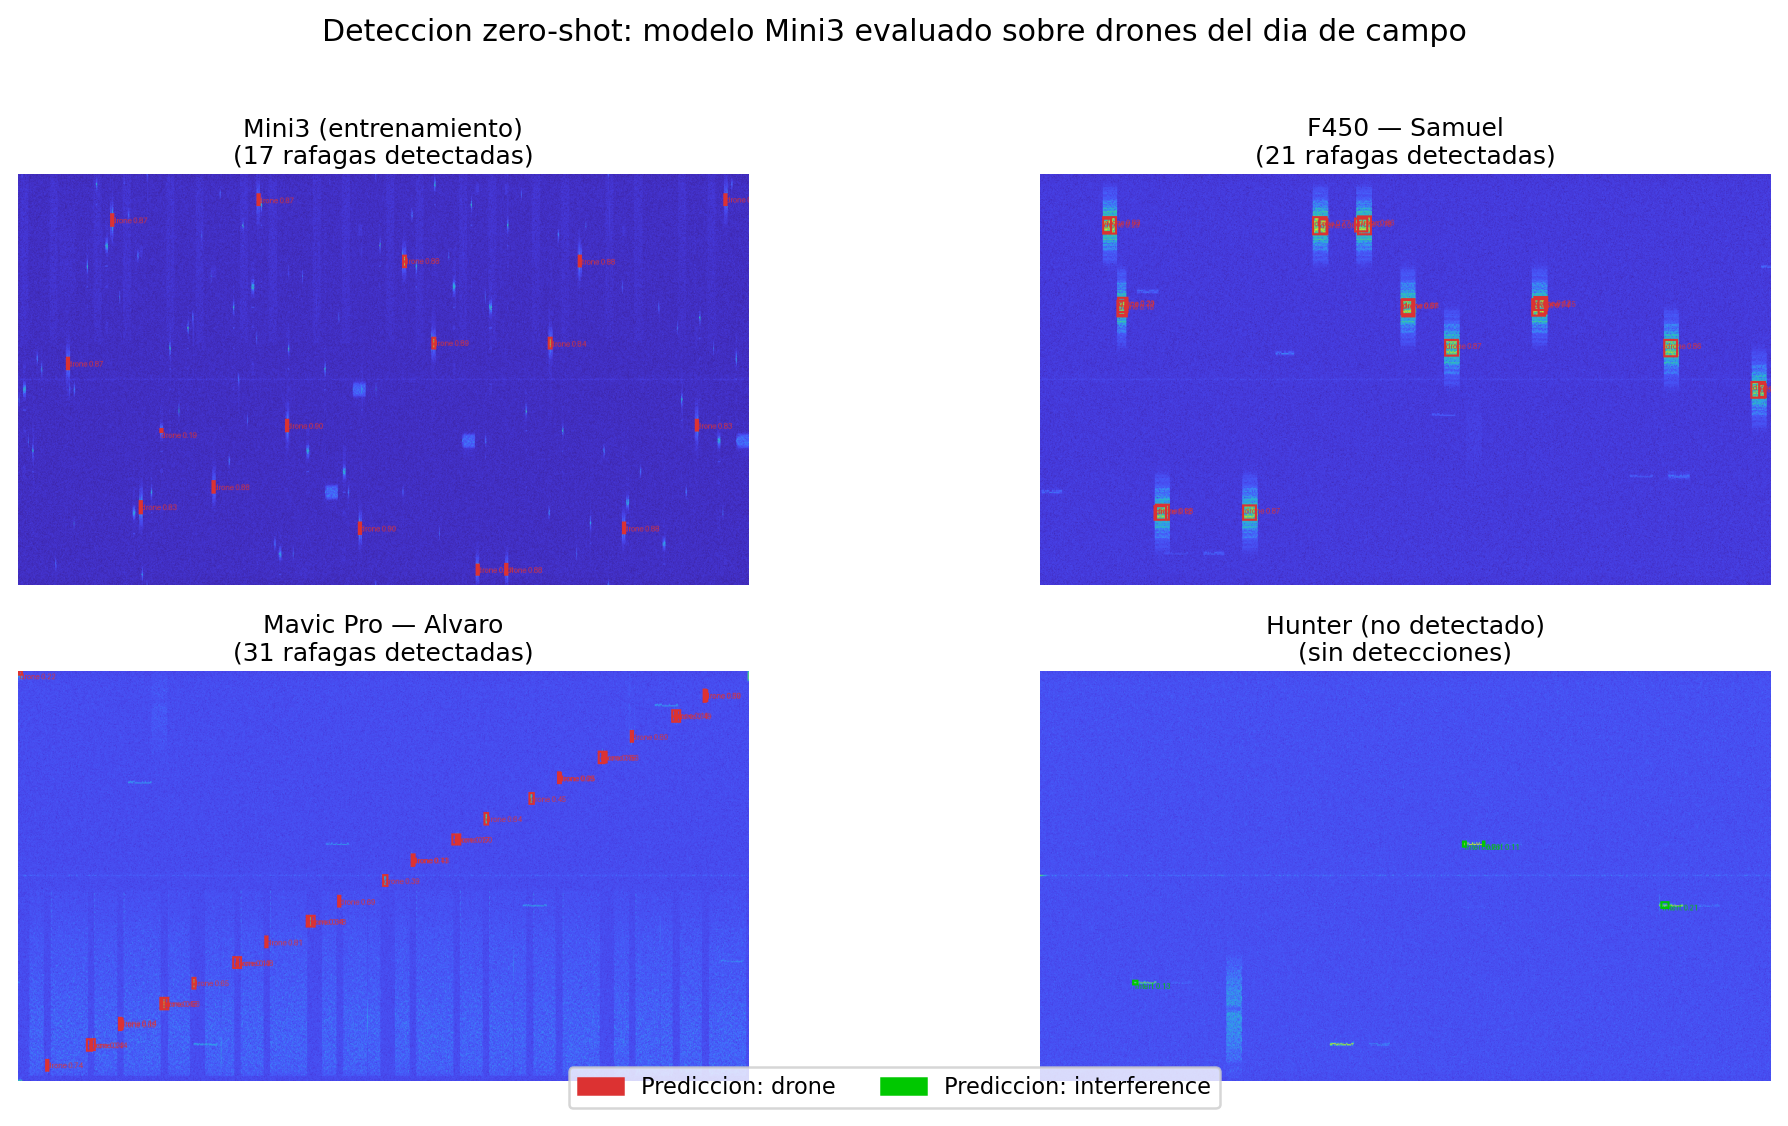
\includegraphics[width=\textwidth]{figuras/resultados/zeroshot_comparativa.png}
    \caption{Detección sobre drones no vistos en el entrenamiento. Para cada plataforma se muestra un espectrograma con las predicciones del detector superpuestas (rojo: \emph{drone}; verde: \emph{interference}). En el Mini~3 (referencia), el F450 y el Mavic~Pro el detector marca en rojo las ráfagas FHSS. En el Hunter no emite ninguna caja de dron, porque su señal no presenta esa morfología.}
    \label{fig:zeroshot_comparativa}
\end{figure}

\FloatBarrier
\subsection{Estadísticas: cuántas ráfagas detecta en cada dron}
\label{sec:zeroshot_estadisticas}

Para cuantificar el comportamiento basta con contar, de media, cuántas ráfagas de dron detecta en cada imagen y en qué porcentaje de imágenes confirma la presencia del dron (criterio de presencia con al menos una ráfaga, igual que en P3). La \cref{tab:zeroshot} resume el resultado sobre los más de \num{1800}~espectrogramas de los tres drones, y la \cref{fig:zeroshot_recall} lo representa gráficamente.

\begin{table}[htbp]
\centering
\caption{Resultado de la prueba de generalización sobre drones no vistos. La media de ráfagas es el número medio de cajas \emph{drone} por espectrograma; el recall de presencia es el porcentaje de imágenes en las que se confirma el dron.}
\label{tab:zeroshot}
\begin{tabular}{lcccc}
\toprule
\textbf{Dron} & \textbf{Protocolo} & \textbf{Imágenes} & \textbf{Ráfagas/imagen} & \textbf{Recall (\%)} \\
\midrule
DJI Mini~3 (ref.) & OcuSync~v2   & ---  & ---   & 99,0  \\
DJI F450          & OcuSync~v1   & 224  & 11,5  & 100,0 \\
Mavic~Pro         & OcuSync~v1   & 874  & 10,2  & 94,2  \\
Hunter            & Desconocido  & 788  & 0,0   & 0,5   \\
\bottomrule
\end{tabular}
\end{table}

\begin{figure}[htbp]
    \centering
    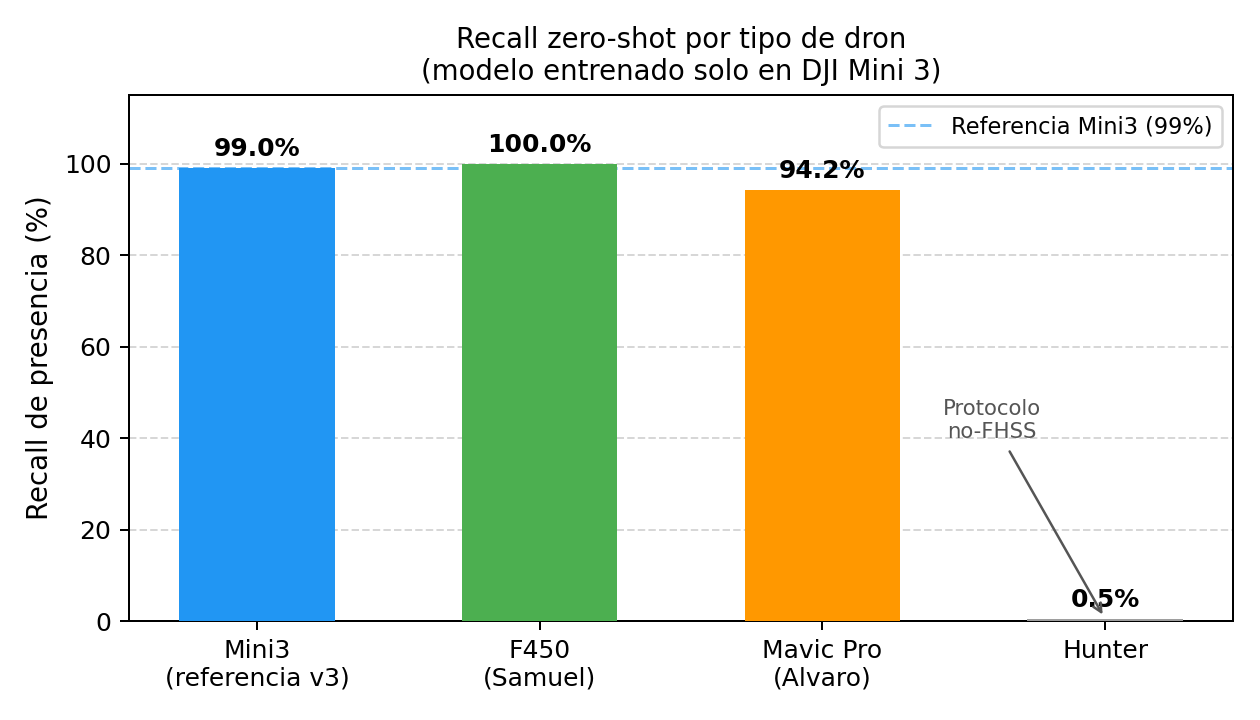
\includegraphics[width=0.8\textwidth]{figuras/resultados/zeroshot_recall_barras.png}
    \caption{Porcentaje de imágenes en las que el detector ---entrenado solo con el Mini~3--- confirma la presencia de dron, para cada plataforma. El F450 y el Mavic~Pro alcanzan el nivel de la referencia del Mini~3; el Hunter se queda en el \SI{0,5}{\percent} por no emitir señal FHSS.}
    \label{fig:zeroshot_recall}
\end{figure}

Los dos drones con protocolo OcuSync~v1 (F450 y Mavic~Pro) se comportan como el Mini~3: detecta en ellos una decena de ráfagas por imagen y confirma su presencia en casi todas las ventanas, sin reentrenamiento y pese a la diferencia de frecuencia. El Hunter, por el contrario, queda prácticamente sin detecciones de dron.

\FloatBarrier
\subsection{Por qué el detector no ve al Hunter}
\label{sec:zeroshot_hunter}

El fallo en el Hunter no es un error del detector, sino la consecuencia esperable de su criterio. El Hunter no transmite mediante saltos de frecuencia: su señal es de espectro ensanchado continuo (compatible con DSSS o un esquema propietario), sin las ráfagas compactas y separadas que caracterizan a OcuSync. Como el detector aprendió a buscar precisamente esa forma ---columnas cortas y aisladas en el plano tiempo-frecuencia--- y el Hunter no la presenta, no encuentra nada que marcar como dron.

Conviene subrayar un matiz: el detector no ignora la señal del Hunter, sino que la \emph{ve} y la clasifica como \emph{interference}. De hecho emite una media de \num{7,5}~cajas de interferencia por espectrograma, con al menos una en la totalidad de las \num{788}~imágenes. Es decir, reconoce que hay una señal activa, pero su morfología no es la de un salto FHSS, así que la asigna a la clase de interferencia y no a la de dron. El Hunter queda, por tanto, fuera del dominio para el que el sistema fue diseñado: el detector está pensado para señales FHSS, y el Hunter no lo es.

Este resultado, lejos de ser un punto débil, es la prueba más clara de qué ha aprendido el modelo. El detector reconoce la morfología FHSS allí donde aparece ---en drones distintos, con protocolos distintos y en frecuencias distintas--- y deja de detectar únicamente cuando esa morfología no existe. No ha memorizado al DJI~Mini~3: ha aprendido a reconocer la huella que deja un salto de frecuencia.

\subsection{Alcance del experimento: capturas de señal limpia}
\label{sec:zeroshot_alcance}

Conviene interpretar estas cifras tan altas en su justo contexto. Las capturas de campo de los tres drones se realizaron, en su mayoría, en condiciones de \emph{señal limpia}: con el dron como emisor dominante, a distancias moderadas y sin inyección de ruido ni interferencia intensa que solapara con sus ráfagas. Este experimento no pretende medir la robustez del detector frente al ruido ---esa cuestión se aborda por separado en el barrido de SNR del experimento P4---, sino responder a una pregunta más concreta: ¿reconoce el detector la morfología FHSS de un dron que nunca ha visto cuando esa morfología es claramente visible en el espectrograma? Para aislar esa pregunta es necesario, precisamente, partir de capturas en las que la firma del dron no esté enmascarada.

Por ello, los recall cercanos al \SI{100}{\percent} del F450 y el Mavic~Pro deben leerse como el rendimiento del detector en condiciones favorables, no como una garantía de comportamiento en cualquier escenario. En un despliegue real ---con interferencia WiFi y Bluetooth densa, mayores distancias, ángulos de antena desfavorables o niveles de señal más bajos--- es esperable que el recall descienda, igual que ocurría en el dataset~v3 del Mini~3 con las capturas más difíciles. El único indicio en esa dirección dentro de este experimento son las dos sesiones del Mavic~Pro con señal débil y las capturas con WiFi denso, donde el rendimiento ya muestra cierta sensibilidad a las condiciones de captura.

En resumen, lo que demuestra este experimento es la \emph{capacidad de transferencia} del detector a drones nuevos cuando la señal es observable, no su robustez en condiciones adversas. Ambas propiedades son necesarias para un sistema de vigilancia completo, pero se validan con experimentos distintos: la transferencia aquí, y la robustez frente al ruido en P4. La validación conjunta ---drones no vistos \emph{y} en condiciones de interferencia controlada--- requiere un conjunto de datos específico y queda planteada como trabajo futuro (dataset~v4).
